\graphicspath{{./}{./figures/}{./figures/spiegelib/}}

\chapter{SpiegeLib: A framework for automatic synthesizer research}
\label{chapter:spiegelib}

This chapter introduces SpiegeLib, a software framework for automatic synthesizer programming  research that was developed by the author as a component of this thesis. SpiegeLib is an open-source software library written in the Python programming language with the goal of promoting collaboration and reproducibility in automatic synthesizer research. The development of the library was based on work published by Yee-King \textit{et al.} \cite{yee2018automatic} that explored automatic synthesizer programming of a VST FM synthesizer using deep learning methods. In their work they focused on the inverse synthesis problem which has the goal of finding synthesizer parameters to match a target sound, also referred to as sound matching. SpiegeLib is designed to support research in inverse synthesizer and provide a platform for sharing and evaluating methods.

Vandewalle \textit{et al.} argue that reproducibility in computational science research increases the impact of a work and they provide a framework for evaluating the quality of reproducibility \cite{vandewalle2009reproducible}. The aim of SpiegeLib is to provide a platform for researchers of automatic synthesizer programming to develop, test, and share implementations in a way that promotes reproducibility at the highest level. SpiegeLib stands for Synthesizer Programming with Intelligent Exploration, Generation, and Evaluation Library. The name SpiegeLib was chosen to pay homage to Laurie Spiegel, an early pioneer in electronic music composition. Laurie Spiegel is known for utilizing synthesizers and software to automate certain aspects of the music composition process. Her philosophy for using technology in music serves as a motivation for the SpiegeLib software library: ``I automate whatever can be automated to be freer to focus on those aspects of music that can't be automated. The challenge is to figure out which is which." \cite{hinkle2006women}

\section{Open Source Research Software}
 In Vandewalle \textit{et al.}'s paper on reproducibility in computational sciences, they advocate for providing other researchers with ``all the information (code, data, schemes, etc.) that was used to produce the presented results"\cite{vandewalle2009reproducible}. Several authors of automatic synthesizer programming research have started to make their work open-access with source code available online. 
 
 Martin Roth and Matthew Yee-King developed $JVstHost$, a Java-based Virtual Studio Technology (VST) plugin host that was published by Matthew Yee-King \cite{yee2011automatic} and was a component of $SynthBot$ \cite{yee2008synthbot}. However, the code for $SynthBot$ itself was not released. Matthew Yee-King also shared the source code for $EvoSynth$, an application for interactive synthesizer patch exploration \cite{yee2016use}. A version of $EvoSynth$ is hosted online allowing for immediate experimentation\footnote{\url{http://www.yeeking.net/evosynth/}}. Krekovi{\'c} \textit{et al.} released source code for their $MightyKnob$ system \cite{krekovic2016algorithm}. Esling \textit{et al.} released open-source code and a Max4Live\footnote{\url{https://www.ableton.com/en/live/max-for-live/}} application for $FlowSynth$ \cite{esling2020flow}. Le Vaillant \textit{et al.} released source code for their generative VAE model\footnote{\url{https://github.com/gwendal-lv/preset-gen-vae}} for performing inverse synthesis with Dexed \cite{le2021improving}. Yee-King \textit{et al.} recently took initial steps towards a software framework for automatic synthesizer programming research with the release of source code that provides functionality for generating research datasets and a set of algorithms for parameter estimation \cite{yee2018automatic}. Along with that work they released the $RenderMan$\footnote{\url{https://github.com/fedden/RenderMan}} library for programmatically interacting with VST synthesizers using the Python programming language.
 
 SpiegeLib builds upon this work with the goal of supporting and encouraging reproducibility within the automatic synthesizer programming research community. SpiegeLib is inspired by the steps that Yee-King \textit{et al.} took towards creating a software library for automatic synthesizer programming research and extends that work with the inclusion of: an object-oriented API, base classes for customization, more robust evolutionary techniques, basic subjective evaluation, complete documentation, and packaging and delivery. It provides a framework for authors to share implementations in an open-access way that allows other researchers to quickly recreate results using a clearly documented set of freely-available tools.
 
\section{Design of SpiegeLib}
\label{chapter:inverse_synth;section:spiegelib}

SpiegeLib is designed to be as extensible as possible to allow researchers to develop and test new implementations of components for conducting automatic synthesizer programming research. There are several stages in a typical automatic synthesizer programming experiment:

\textbf{1) Synthesizer configuration}: a synthesizer is selected and a subset of the parameters may be selected for estimation. For example, in work by Yee-King \textit{et al.} \cite{yee2018automatic}, several different experiments were conducted using successively larger parameter subsets to increase the difficulty.

\textbf{2) Dataset generation}: for experiments requiring training, such as learning deep learning models, a dataset of synthesized audio and parameter pairs must be generated. Audio features may be extracted at this point too, which will be used as input to a model.

\textbf{3) Training models}: deep learning models are trained using the generated dataset.

\textbf{4) Sound matching}: this is the stage where parameters are estimated to match a target sound. In the case of deep learning models this involves inferring parameters using the trained model. For search techniques, the algorithm is run using the target audio as input.

\textbf{5 Evaluation}: results of the sound matching are evaluated here. Objective evaluation can be performed directly on the parameters as was the case in work by Barkan \textit{et al.} \cite{barkan2019inversynth},  or audio can be rendered using the predicted parameters and evaluation carried out on the audio, which was done by both Barkan \textit{et al.} and Yee-King \textit{et al.} \cite{yee2018automatic}. Subjective evaluation can also be carried out at this point with a user listening experiment.

SpiegeLib contains components to support all stages of this experimental pipeline. Implementation details and the components of the library are detailed in the following section.

% - Figure for the research pipeline?

\section{Library Components}

Base classes with functionality for interacting with software synthesizers, audio feature extraction, parameter estimation, and evaluation provide an API to support development of custom implementations that will work with other components of the library. A number of utility classes are also provided for handling audio signals, generating datasets, and running experiments.

SpiegeLib is written in the Python programming language and utilizes Python packages common in research including \mintinline{python}{numpy}, \mintinline{python}{scipy}, \mintinline{python}{tensorflow}, and \mintinline{python}{librosa}. SpiegeLib itself is a python package and is available through the Python Package Index (PyPI) with pip\footnote{\url{https://pypi.org/}}. All dependencies, except for \mintinline{python}{librenderman}, are python packages available through the PyPI and will be automatically installed by pip. For more information on installation, system requirements, and detailed library documentation, please refer to the  online documentation.\footnote{\url{https://spiegelib.github.io/spiegelib/}}

A summary of the currently implemented algorithms is shown in table \ref{table:spiegel_algorithms}. A brief overview of these components and the main classes and functionalities of SpiegeLib is provided in the following sections.
 
\begin{table*}[t]
\centering\small
\begin{threeparttable}
	\caption{Algorithms currently implemented as classes in \mintinline{python}{spiegelib}}
	\label{table:spiegel_algorithms}
	\begin{tabular}{|c|c|c|}
	\hline
	\multicolumn{3}{|c|}{\textbf{Algorithms in \mintinline{python}{spiegelib}}} \\
	\hline
	\hline
	\textbf{Feature Extraction} & \textbf{Deep Learning Estimators} & \textbf{Optimization Estimators} \\
	\hline
	FFT 		& MLP \cite{yee2018automatic} 		& Basic GA   			\\
	STFT 		& LSTM \cite{yee2018automatic} 		& NSGA III \cite{tatar2016automatic}				\\\cline{3-3}
	MFCC		& LSTM++ \cite{yee2018automatic} 	& \textbf{Objective Evaluation} 	\\\cline{3-3}
	Spectral\tnote{1}	& Conv6 \cite{barkan2019inversynth} 	& MFCC Evaluation 		\\
	\hline
	\end{tabular}
	\begin{tablenotes}[para, flushleft]
			\footnotesize
			\item[1] Spectral bandwidth, centroid, contrast, flatness, and rolloff.
	\end{tablenotes}
\end{threeparttable}
\end{table*}
 
\subsection{AudioBuffer}
The \mintinline{python}{AudioBuffer} class is used to pass audio signal signals throughout the library. It holds an array of audio samples and sample rate information. Methods of the \mintinline{python}{AudioBuffer} class provide functionality for loading audio from a variety of file formats, resampling, normalizing, time segmenting, plotting spectrograms, and saving audio as WAV files.

\subsection{Synthesizers}
The \mintinline{python}{SynthBase} class is an abstract base class that provides an interface for creating programmatic interactions with software synthesizers. \mintinline{python}{SynthBase} stores information and contains methods required for interaction with other components in SpiegeLib, including getting parameter lists, setting and getting patch configurations, overriding/freezing parameters, triggering audio rendering using MIDI notes, getting audio samples as \mintinline{python}{AudioBuffer}s, and requesting randomized patch settings. All patch settings are stored as a list of parameter tuples which contain the parameter number and parameter value. All parameter values are expected to be floating point numbers in the range [0.0, 1.0]. No requirement is made on how underlying synthesis engines are implemented, however, inheriting classes must provide parameter descriptions in a class attribute during construction and must provide implementations for four abstract class methods related to loading patches, randomizing patches, rendering audio, and returning an \mintinline{python}{AudioBuffer} of rendered audio.

%
% \mintinline{python}{load_patch()}, \mintinline{python}{randomize_patch()}, \mintinline{python}{render_patch()}, and \mintinline{python}{get_audio()}.

\mintinline{python}{SynthVST} is an implementation of \mintinline{python}{SynthBase} and provides an interface for interacting with VST synthesizers. \mintinline{python}{SynthVST} is a wrapper for the $RenderMan$ Python library developed by Leon Fedden in conjunction with research by Yee-King \textit{et al.} \cite{yee2018automatic}.

\subsection{Audio Feature Extraction}
The abstract base class \mintinline{python}{FeaturesBase} provides an interface for computing audio representations and extracting features from raw audio samples. The \mintinline{python}{getFeatures()} abstract method must be overridden in inheriting classes and is where feature extraction algorithms are run.  \mintinline{python}{FeatureBase} also includes functionality for standardizing results. By default, data is standardization is computing by removing the mean and scaling to unit variance. Parameters for standardization can be set based on the distribution from one dataset, saved, reloaded, and applied to new results to ensure that standardization is carried out using the same parameters. Currently, implemented feature extraction classes utilize the \mintinline{python}{librosa} library \cite{mcfee2015librosa} and include Mel Frequency Cepstral Coefficients (\mintinline{python}{MFCC}), Short Time Fourier Transform (\mintinline{python}{STFT}), Mel-Spectrograms (\mintinline{python}{MelSpectrogram}), Fast Fourier Transform (\mintinline{python}{FFT}), and a set of time summarized spectral features (\mintinline{python}{SpectralSummarized}).

\subsection{Datasets}
The \mintinline{python}{DatasetGenerator} class provides functionality for creating datasets of audio samples, feature vectors, and associated parameter settings from a synthesizer. An implementation of \mintinline{python}{SynthBase} and \mintinline{python}{FeaturesBase} are passed in as arguments to the \mintinline{python}{DatasetGenerator} constructor. To generate a dataset, random patches for the synthesizer are created and feature extraction is performed on the resulting audio. In this way, datasets for training and validating deep learning models, as well as datasets for evaluating sound matching experiments can be automatically generated. 
%The term contrived in the context of automatic synthesizer programming research refers to the use of audio samples produced by the synthesizer being studied as a target for sound matching \cite{justice1979analytic}. The benefit of using a contrived sound for evaluation is that it minimizes the uncertainty regarding whether the synthesizer in question is capable of producing the target sound. 
External datasets can also be used within SpiegeLib and the \mintinline{python}{AudioBuffer} class provides support for loading folders of audio samples for processing.

\subsection{Estimators}
All parameter estimation classes implement the \mintinline{python}{EstimatorBase} abstract base class. \mintinline{python}{EstimatorBase} is a minimal base class with one abstract method, \mintinline{python}{predict()}, that has an optional input argument. Implementations of estimators are split into deep learning approaches and other approaches including evolutionary algorithms.  The included algorithms do not represent a comprehensive set of methods for automatic synthesizer programming research but are meant to cover common methods informed by previous work. Ten estimators are currently implemented and the author plans to add more in the near future including: a hill climbing optimizer \cite{yee2018automatic}, a particle swarm optimizer \cite{heise2009automatic}, a 1D CNN for raw audio input \cite{barkan2019inversynth}, and recent generative approaches \cite{esling2020flow, le2021improving}.

\subsection{Deep Learning Estimators}
All deep learning models are implementations of the \mintinline{python}{TFEstimatorBase} abstract base class which utilizes the \mintinline{python}{tensorflow}\footnote{\url{https://www.tensorflow.org}} and \mintinline{python}{keras}\footnote{\url{https://www.tensorflow.org/guide/keras}} machine learning libraries. \mintinline{python}{TFEstimatorBase} implements \mintinline{python}{EstimatorBase} and provides wrapper functions for setting up data for training and validation, training models, running predictions, and saving and loading model weights. While these methods are designed to help in handling of data typical to a synthesizer parameter estimation problem, all methods for a \mintinline{python}{tf.keras.Model} can be accessed directly from the \mintinline{python}{model} class member. Classes that inherit from \mintinline{python}{TFEstimatorBase} define models in an implementation of the \mintinline{python}{buildModel()} method which is automatically called during construction in the base class. This allows new models to be quickly designed, switched out, and compared with minimal effort.

The currently implemented deep learning models are based on prior work, specifically on work on Recurrent Neural Networks by Yee-King \textit{et al.} \cite{yee2018automatic} and work on Convolutional Neural Networks (CNN) by Barkan \textit{et al.} \cite{barkan2019inversynth}. Two modified CNN models with reduced capacity are also included (\mintinline{python}{Conv6s} and \mintinline{python}{Conv5s}). These models were created during the experiments conducted in chapter \ref{chapter:inverse_synth_experiment} and were found to result in more stable training for synthesizers with less parameters. For a full listing of deep learning models implemented, see table \ref{table:spiegel_algorithms}. An example code listing of sound matching using a trained LSTM model is shown in figure \ref{fig:lstm_code}.

To save training and validation progress, the \mintinline{python}{TFEpochLogger} class can be passed in as a callback during model training. \mintinline{python}{TFEpochLogger} stores training accuracy and loss, and validation accuracy and loss over training epochs in a dictionary object which can be plotted after training.

%Example code listing
\begin{figure}[t]
\centering
\footnotesize
\begin{minted}{python}
import spiegelib as spgl
import spiegelib.estimator.TFEstimatorBase

# Load VST and set parameters from JSON file
synth = spgl.synth.SynthVST('./Dexed.vst')
synth.load_state('./dexed_simple_fm.json')

# MFCC Audio Feature Extractor
ftrs = spgl.features.MFCC(normalize=True)

# Load saved normalization parameters
ftrs.load_normalizers('./normalizers.pkl')

# Load LSTM model from saved model file
lstm = TFEstimatorBase.load('./fm_lstm.h5')

matcher = spgl.SoundMatch(synth, lstm, ftrs)

target = spgl.AudioBuffer('./target.wav')
output = matcher.match(target)
output.save('./lstm_predicted_audio.wav')
\end{minted}
\caption{Example of SpiegeLib performing a sound match from a target WAV file on a VST synthesizer. A pre-trained LSTM deep learning model is used with MFCC input.}
\label{fig:lstm_code}
\end{figure} 

\subsection{Search-based Estimators}
Two search-based estimators are currently implemented and utilize the DEAP python library \cite{fortin2012deap}. A basic GA (\mintinline{python}{BasicGA}) is included as well as a multi-objective non-dominated sorting genetic algorithm III (\mintinline{python}{NSGA3}). Both GAs require feature extraction objects, or a list of feature extraction objects in the case of the multi-objective algorithm, which are used in the GA evaluation function.

\subsection{Hybrid Estimator}
A parameter estimation technique that is introduced as a part of this thesis is also included in SpiegeLib. This estimator uses a pre-trained deep learning network during the initial population generation for an NSGA-III algorithm. The goal of this approach, which is explored in more depth in the next chapter, is to provide a warm start for the genetic algorithm search with the intention of enabling it find a suitable solution in less generations. As such, this estimator is called a Warm-Start NSGA-III, or WS-NSGA3 (\mintinline{python}{WSNSGA3}).

\subsection{Evaluation}
Objective evaluation of results can be carried out by measuring error between audio samples. \mintinline{python}{EvaluationBase} is an abstract base class for calculating evaluation metrics on a set of target and prediction data. A list of target values and lists of predictions for each target are passed into the constructor. \mintinline{python}{EvaluationBase} provides functionality for calculating statistics on results, saving results as a JSON file, plotting results in histograms, and calculating metrics including mean absolute error, mean squared error, euclidean distance, and manhattan distance. Inheriting classes must implement the \mintinline{python}{evaluate_target()} method which is called for each target and associated estimations and is expected to return a dictionary of metrics for each estimation. The \mintinline{python}{MFCCEval} class implements \mintinline{python}{EvaluationBase} and calculates metrics on MFCC vectors for targets and estimations; the \mintinline{python}{LSDEval} class calculates the Log Spectral Distance (LSD) between two audio files; and the \mintinline{python}{ParameterEval} class calculates absolute error on each parameter separately, as well as the mean absolute error across all parameter values.

Functionality for conducting subjective evaluation of results is provided in the \mintinline{python}{BasicSubjective} class. This class accepts a set of audio files and runs a locally hosted server that generates a simple web interface using BeaqleJS \cite{kraft2014beaqlejs}. An image of this interface is shown in figure \ref{fig:basic_subjective}. This runs a MUSHRA style listening test, where stimuli are ranked in terms of match quality to a reference.  For inverse synthesis experiments, audio targets can be passed in along with a set of predictions for each target, and a sound similarity test will be generated with options for randomizing the ordering of targets and predictions. Results can then be saved as a JSON file.

\begin{figure}
    \centering
    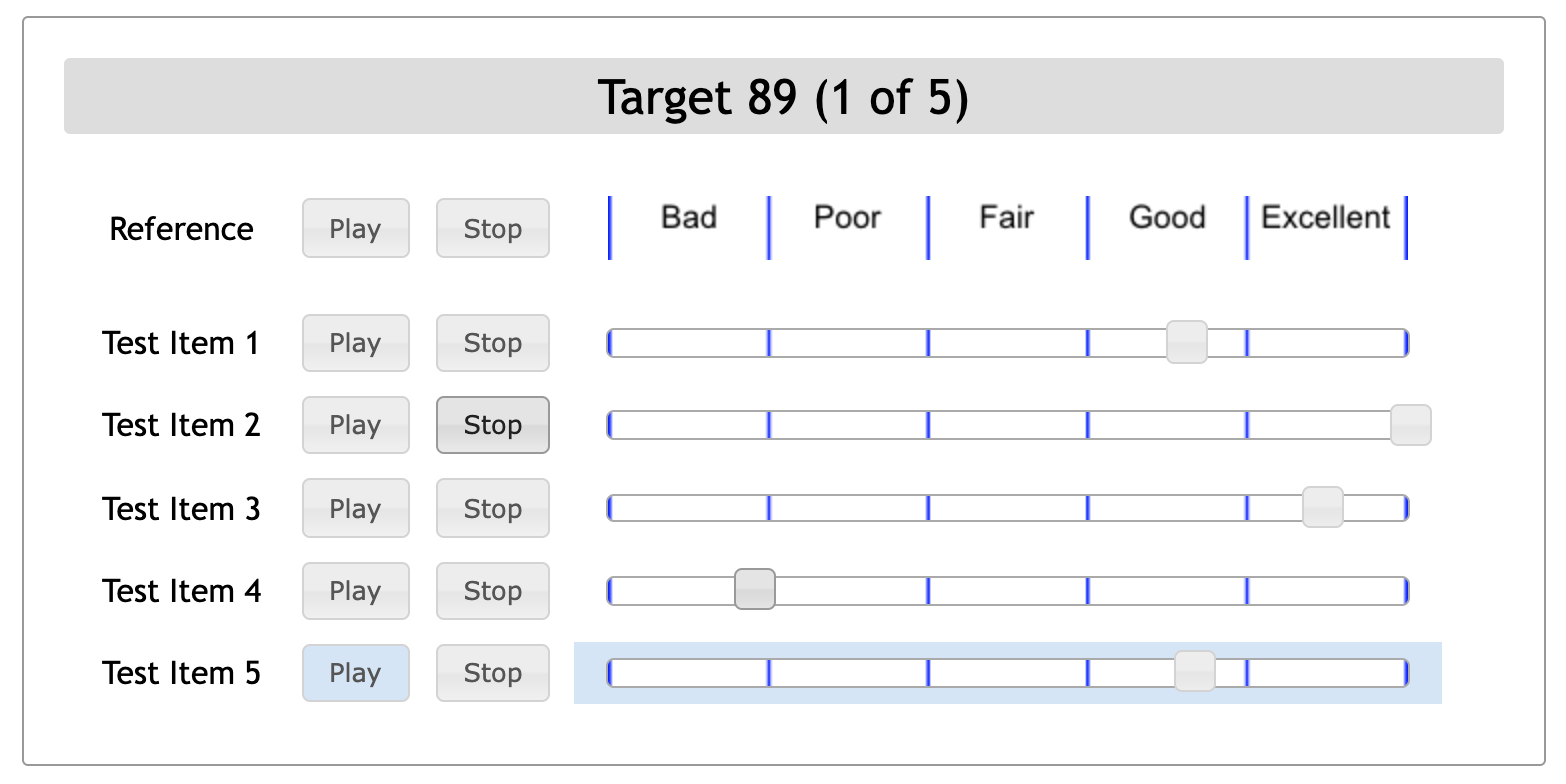
\includegraphics[width=0.9\textwidth]{figures/spiegelib/beaqlejs_interface.png}
    \caption{Interface for the basic subjective evaluation test using BeaqleJS. This is a MUSHRA style test. Results from four different estimators are being compared. A hidden reference is also included in the test items. The user must rank the quality of each test item against the reference (target used for inverse synthesis).}
    \label{fig:basic_subjective}
\end{figure}

%TODO: Add in a visual of this? What did we use to create this?

% \subsection{Helper Classes}
% - What other classes are available in SpiegeLib that we should comment on?

% mintinline{python}{SoundMatch} is a functional class that uses an estimator to predict synthesizer parameter settings for an implementation of \mintinline{python}{SynthBase} in order to match a target sound.


\section{Future Work and Conclusion}
Development of SpiegeLib is ongoing and a number of expansions to the current library are planned. First, the author would like to continue to expand the number of estimators available and plan on integrating the following: a hill climbing optimizer \cite{yee2018automatic}, a particle swarm optimizer \cite{heise2009automatic}, a 1D CNN for raw audio input \cite{barkan2019inversynth}, and generative approaches \cite{esling2020flow, le2021improving}.  Second, the author would like to expand on the type of interactions available such as automatic programming from vocal imitations \cite{mcartwright2014} and interactive methods. 
%Third, we would like to integrate more sophisticated subjective evaluation tools such as creating links to setup tests using the Web Audio Evaluation Tool \cite{waet2015}. Third, we would like to contribute to the $RenderMan$ library that is used in this work in order to extend support to Windows users and distribute the library via PyPI so the entire SpiegeLib library can be installed in one command. 
Finally, the author would like to encourage developers and researchers from the automatic synthesizer programming community to contribute to SpiegeLib. Information on contributing is available online.\footnote{\url{https://spiegelib.github.io/spiegelib/contributing.html}} 

This chapter has introduced SpiegeLib, an open-source automatic synthesizer programming library. SpiegeLib is an object-oriented software library that was designed with the goal of supporting development, collaboration, and reproducibility in the field. The library includes implementations of classes for conducting automatic synthesizer programming research. These classes contain functionality for interacting with VST synthesizers, extracting audio features, creating datasets, estimating synthesizer parameters, and evaluating results. Ten implementations of deep learning and evolutionary parameter estimation techniques based on previous work are included, with more planned.